% dvisvgm --pdf name
% latexmk -C
\documentclass[preview]{standalone}
\usepackage{tikz}
\usepackage{amsmath}
\usepackage{color}
\usepackage{tabularray}
\definecolor{Sushi}{rgb}{0.545,0.756,0.294}
\definecolor{Frost}{rgb}{0.933,0.968,0.89}
\usetikzlibrary{shapes.geometric, arrows}
\tikzstyle{block} = [rectangle, rounded corners,
minimum width=3.5cm,
minimum height=2cm,
text centered, 
draw=gray]

\tikzstyle{io} = [trapezium, 
trapezium stretches=true,
trapezium left angle=70, 
trapezium right angle=110, 
minimum width=3.5cm, 
minimum height=2cm, text centered, 
draw=gray]

\tikzstyle{process} = [rectangle, 
minimum width=3.5cm,
minimum height=2cm,
text centered, 
text width=3cm, 
draw=gray]

\tikzstyle{decision} = [diamond, 
minimum width=3cm, 
minimum height=1cm, 
text centered, 
draw=gray]
\tikzstyle{arrow} = [thick,->,>=stealth]

\tikzstyle{circ} = [circle, 
minimum size=1cm, 
text centered, 
draw=gray]

\begin{document}
    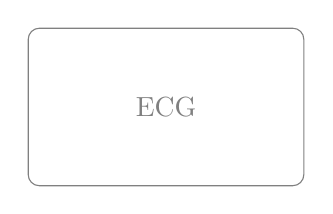
\begin{tikzpicture}[transform shape, every node/.append style={}, color=gray, node distance = 3.5cm]
        % All blocks
        \node (ECG) [block] {ECG};

        
    \end{tikzpicture}
\end{document}